\documentclass[12pt,a4paper]{article}

\usepackage[margin=1in]{geometry}
\usepackage{graphicx}
\usepackage{setspace}
\usepackage{times}
\usepackage{titlesec}
\usepackage{amsmath, amssymb, amsthm}
\usepackage{booktabs}
\usepackage{array}
\usepackage{hyperref}
\usepackage{enumitem}
\usepackage{fancyhdr}
\usepackage{indentfirst}
\usepackage{tikz}
\usetikzlibrary{shapes.geometric, arrows.meta, positioning}
\usepackage{pgfplots}
\pgfplotsset{compat=1.16}
\usepackage{pgfplotstable}
\usepackage{listings}
\usepackage{caption}

\hypersetup{
	colorlinks=true,
	linkcolor=black,
	citecolor=black,
	urlcolor=blue
}

\onehalfspacing
\setlength{\parindent}{0.5in}
\setlength{\parskip}{0pt}

\titleformat{\section}
{\normalfont\bfseries\large}{\thesection.}{0.5em}{}
\titleformat{\subsection}
{\normalfont\bfseries}{\thesubsection.}{0.5em}{}

\pagestyle{fancy}
\fancyhf{}
\fancyhead[L]{Laplace Transform and Error Function Integrals}
\fancyhead[R]{\thepage}
\renewcommand{\headrulewidth}{0.4pt}
\setlength{\headheight}{14.5pt}

\theoremstyle{definition}
\newtheorem{definition}{Definition}[section]
\newtheorem{example}{Example}[section]
\theoremstyle{plain}
\newtheorem{theorem}{Theorem}[section]
\newtheorem{lemma}[theorem]{Lemma}
\newtheorem{corollary}[theorem]{Corollary}
\theoremstyle{remark}
\newtheorem{remark}{Remark}[section]

\newcommand{\erf}{\operatorname{erf}}
\newcommand{\erfc}{\operatorname{erfc}}
\newcommand{\Lap}[1]{\mathcal{L}\!\left\{#1\right\}}
\newcommand{\dd}{\,\mathrm{d}}

\newcommand{\UniversityName}{Bulacan State University}
\newcommand{\CollegeName}{College of Science}
\newcommand{\CourseCode}{TWM 301}
\newcommand{\CourseDescription}{Technical Writing (for BS Mathematics)}
\newcommand{\AcademicYear}{Academic Year 2026--2027}
\newcommand{\StudyTitle}{Peer Reviewed Application of Laplace Transform for Solving Improper Integrals whose Integrand Consisting Error Function}
\newcommand{\AuthorNames}{Angel Germino \\ Sabrina Bianca Concepion \\ Randy Jr. B. Poling \\ Emmanuel Joseph R. Vendivil}
\newcommand{\CourseYearSection}{BS Mathematics Major in Business Application 3A}
\newcommand{\InstructorName}{Aarhus M. Dela Cruz}
\newcommand{\SubmissionDate}{\today}

\newcommand{\BulSULogo}{bulsu.png}
\newcommand{\CSLogo}{college_of_science.png}

\lstset{
	basicstyle=\ttfamily\footnotesize,
	breaklines=true,
	frame=single,
	columns=fullflexible,
	keepspaces=true,
	language=[LaTeX]TeX,
	showstringspaces=false
}

\begin{document}
	
	\begin{titlepage}
		\centering
		
		\vspace*{0.3in}
		
		\begin{minipage}{0.22\textwidth}
			\centering
			\includegraphics[width=0.95\linewidth]{\BulSULogo}
		\end{minipage}
		\hfill
		\begin{minipage}{0.50\textwidth}
			\centering
			{\Large\bfseries \UniversityName\par}
			\vspace{0.15cm}
			{\large\bfseries \CollegeName\par}
			\vspace{0.15cm}
			{\normalsize \CourseCode: \CourseDescription\par}
			\vspace{0.15cm}
			{\normalsize \AcademicYear\par}
		\end{minipage}
		\hfill
		\begin{minipage}{0.22\textwidth}
			\centering
			\includegraphics[width=0.95\linewidth]{\CSLogo}
		\end{minipage}
		
		\vspace{1.2in}
		
		{\Large\bfseries MINI RESEARCH AND EXPOSITION PAPER\par}
		
		\vspace{0.6in}
		
		{\Large\bfseries \StudyTitle\par}
		
		\vspace{0.9in}
		
		{\large\bfseries Authors\par}
		\vspace{0.2cm}
		{\large \AuthorNames\par}
		
		\vspace{0.6in}
		
		{\large \CourseYearSection\par}
		
		\vfill
		
		{\normalsize Submitted to:\par}
		\vspace{0.15cm}
		{\normalsize\bfseries \InstructorName\par}
		
		\vspace{0.4in}
		
		{\normalsize \SubmissionDate\par}
	\end{titlepage}
	
	\pagenumbering{roman}
	\setcounter{page}{1}
	
	\begin{abstract}
		\noindent This paper presents an exposition and critical peer review of the article ``Application of Laplace Transform for Solving Improper Integrals whose Integrand Consisting Error Function'' by Aggarwal et al.\ (2019). The paper re-derives the Laplace transform of $\erf(\sqrt{t})$ by two routes: a term-by-term Maclaurin series, which is valid for $s>1$, and an integral-representation argument, which is valid for all $s>0$. The result, $1/\bigl(s\sqrt{s+1}\bigr)$, is combined with the shifting, change-of-scale, differentiation, integration, multiplication-by-$t$, and convolution properties to evaluate six improper integrals involving the error function. Each exact value is compared with independent adaptive numerical quadrature and agrees to at least six significant digits. The truncation error of the series is analysed through the alternating-series bound. The review identifies several flaws in the article: an incorrect limit for the complementary error function, an incorrect expression for $\Lap{t\,\erf(\sqrt{t})}$, a misstated change-of-scale property, missing convergence conditions on the parameter $s$, and an inconsistent issue number. The worked results themselves are correct. The paper concludes that the Laplace-transform method is an exact and economical alternative to direct integration, provided that the region of convergence is stated and checked.
	\end{abstract}
	
	\noindent\textbf{Keywords:} Laplace transform, error function, complementary error function, improper integrals, convolution theorem, convergence
	
	\newpage
	\tableofcontents
	\listoffigures
	\listoftables
	\newpage
	
	\pagenumbering{arabic}
	\setcounter{page}{1}
	
	\section{Introduction}
	
	\subsection{Background and Motivation}
	
	Improper integrals over unbounded intervals appear throughout probability, physics, and engineering. Many of them yield to elementary techniques, but those whose integrands contain a special function often do not. The error function is a prominent example. It arises in heat conduction, mass transfer, vibrating-beam problems, and the normal distribution (Aggarwal et al., 2019), and it has no elementary antiderivative. Integrals such as $\int_0^\infty e^{-t}\erf(\sqrt{t})\dd t$ therefore cannot be handled by standard substitution or integration by parts.
	
	The Laplace transform offers an alternative. By definition, the transform of a function is itself an improper integral over $[0,\infty)$. If the integrand of a given improper integral can be recognised as $e^{-st}f(t)$ for a function $f$ whose transform is known, the integral equals that transform evaluated at the chosen value of $s$. This observation is the basis of the article by Aggarwal et al.\ (2019), which is the subject of this paper.
	
	The topic belongs to Advanced Calculus because it relies on improper integrals, convergence, limits, and series. It also suits a technical writing course, because the correctness of the argument depends on precise statements of definitions, conditions, and notation. Careful reading of a published article shows how small lapses in notation can undermine otherwise sound mathematics.
	
	\subsection{Statement of the Problem}
	
	Aggarwal et al.\ (2019) claim to evaluate six improper integrals containing $\erf(\sqrt{t})$ by Laplace transform techniques. This paper addresses two questions. First, is the method sound, and are the six reported values correct? Second, is the presentation precise enough, in its statements, conditions, and notation, for a reader to rely on it?
	
	\subsection{Objectives of the Paper}
	
	The objectives of this paper are as follows:
	
	\begin{enumerate}[label=\arabic*.]
		\item To introduce the Laplace transform, the error function, and the properties needed to evaluate improper integrals;
		\item To derive the Laplace transform of $\erf(\sqrt{t})$ rigorously and to state the region in which it holds;
		\item To work through the six integrals of Aggarwal et al.\ (2019) and verify each against independent numerical computation;
		\item To assess the accuracy, convergence, and limitations of the method and to document the errors found in the article; and
		\item To summarise the major insights and suggest directions for further study.
	\end{enumerate}
	
	\subsection{Significance, Scope, and Limitations}
	
	The paper shows that a tool usually associated with differential equations also evaluates a particular class of improper integrals exactly. The scope is limited to integrals built from $\erf(\sqrt{t})$ and its variants, as treated by Aggarwal et al.\ (2019). General error-function integrals, other integral transforms, and numerical analysis of the transform inversion are outside the scope. Because the work is analytical, the implementation consists of typeset derivations, plotted functions, and tabulated numerical checks rather than a simulation.
	
	\section{Preliminaries}
	
	This section states the definitions and results used in the rest of the paper. The standard properties of the Laplace transform follow Debnath and Bhatta (2006) and Zill (2016).
	
	\subsection{The Laplace Transform}
	
	\begin{definition}[Laplace transform]\label{def:laplace}
		Let $f$ be defined for $t\ge 0$. The Laplace transform of $f$ is
		\begin{equation}\label{eq:laplace}
			F(s)=\Lap{f(t)}=\int_0^\infty e^{-st}f(t)\dd t,
		\end{equation}
		for those values of $s$ for which the improper integral converges.
	\end{definition}
	
	\begin{theorem}[Existence]\label{thm:existence}
		If $f$ is piecewise continuous on every finite interval $[0,T]$ and of exponential order $\alpha$, that is, $|f(t)|\le Me^{\alpha t}$ for some constants $M$ and $\alpha$ and all large $t$, then $\Lap{f}$ exists for all $s>\alpha$.
	\end{theorem}
	
	These conditions are sufficient but not necessary. Equation~\eqref{eq:laplace} also gives the central principle of this paper.
	
	\begin{remark}[Evaluation principle]\label{rem:principle}
		If $\Lap{f(t)}=F(s)$ is known for $s$ in some interval, then $\int_0^\infty e^{-st}f(t)\dd t=F(s)$ for each $s$ in that interval. An improper integral is therefore evaluated by identifying its integrand as $e^{-st}f(t)$ and substituting the chosen value of $s$ into $F$.
	\end{remark}
	
	\subsection{Properties of the Laplace Transform}
	
	Let $\Lap{f(t)}=F(s)$ and $\Lap{g(t)}=G(s)$. Table~\ref{tab:properties} lists the properties used in this paper. Each holds for $s$ in the common region of convergence.
	
	\begin{table}[htbp]
		\centering
		\caption{Laplace transform properties used in this paper}
		\label{tab:properties}
		\renewcommand{\arraystretch}{1.4}
		\begin{tabular}{l p{7.6cm} l}
			\toprule
			Property & Statement & Used in \\
			\midrule
			Linearity & $\Lap{af+bg}=aF(s)+bG(s)$ & Corollary~\ref{cor:erfc} \\
			First shifting & $\Lap{e^{at}f(t)}=F(s-a)$ & Example~\ref{ex:3} \\
			Change of scale & $\Lap{f(at)}=\tfrac{1}{a}F\!\left(\tfrac{s}{a}\right)$, $a>0$ & Example~\ref{ex:5} \\
			Multiplication by $t$ & $\Lap{t\,f(t)}=-F'(s)$ & Example~\ref{ex:2} \\
			Derivative & $\Lap{f'(t)}=sF(s)-f(0)$ & Example~\ref{ex:5} \\
			Integral & $\Lap{\int_0^t f(u)\dd u}=\tfrac{1}{s}F(s)$ & Example~\ref{ex:4} \\
			Convolution & $\Lap{f*g}=F(s)G(s)$, with $(f*g)(t)=\int_0^t f(x)g(t-x)\dd x$ & Example~\ref{ex:6} \\
			\bottomrule
		\end{tabular}
	\end{table}
	
	The elementary transforms needed are $\Lap{1}=1/s$ for $s>0$ and, for $\nu>-1$,
	\begin{equation}\label{eq:power}
		\Lap{t^{\nu}}=\frac{\Gamma(\nu+1)}{s^{\nu+1}},\qquad s>0,
	\end{equation}
	where $\Gamma(1/2)=\sqrt{\pi}$ and $\Gamma(\nu+1)=\nu\,\Gamma(\nu)$.
	
	\subsection{The Error Function}
	
	The definitions and properties below are standard (Korn \& Korn, 2000).
	
	\begin{definition}[Error and complementary error functions]\label{def:erf}
		\begin{equation}\label{eq:erf}
			\erf(x)=\frac{2}{\sqrt{\pi}}\int_0^x e^{-u^2}\dd u,\qquad
			\erfc(x)=1-\erf(x)=\frac{2}{\sqrt{\pi}}\int_x^\infty e^{-u^2}\dd u.
		\end{equation}
	\end{definition}
	
	\begin{lemma}[Basic properties]\label{lem:erfprops}
		The error function satisfies:
		\begin{enumerate}[label=(\alph*)]
			\item $\erf(0)=0$ and $\erfc(0)=1$;
			\item $\erf(-x)=-\erf(x)$;
			\item $\erf(x)\to 1$ and $\erfc(x)\to 0$ as $x\to\infty$;
			\item $\erf(x)=\dfrac{2}{\sqrt{\pi}}\displaystyle\sum_{k=0}^{\infty}\frac{(-1)^k x^{2k+1}}{k!\,(2k+1)}$ for all real $x$.
		\end{enumerate}
	\end{lemma}
	
	\begin{proof}
		Parts (a) and (b) follow directly from Equation~\eqref{eq:erf}, since the integrand is even. For (c), the Gaussian integral $\int_0^\infty e^{-u^2}\dd u=\sqrt{\pi}/2$ gives $\erf(x)\to 1$, so $\erfc(x)=1-\erf(x)\to 0$. For (d), the Maclaurin series of $e^{-u^2}$ converges uniformly on compact sets and may be integrated term by term.
	\end{proof}
	
	\begin{lemma}[Integral representation]\label{lem:rep}
		For $t\ge 0$,
		\begin{equation}\label{eq:rep}
			\erf(\sqrt{t})=\frac{1}{\sqrt{\pi}}\int_0^t u^{-1/2}e^{-u}\dd u .
		\end{equation}
	\end{lemma}
	
	\begin{proof}
		Substitute $u=x^2$, so that $\dd x=\tfrac{1}{2}u^{-1/2}\dd u$, in $\erf(\sqrt{t})=\tfrac{2}{\sqrt{\pi}}\int_0^{\sqrt{t}}e^{-x^2}\dd x$.
	\end{proof}
	
	\section{Methods and Applications}
	
	\subsection{Model or Method Description}
	
	\subsubsection{Problem setup and assumptions}
	
	The problem is to evaluate improper integrals of the form $\int_0^\infty e^{-st}\,h(t)\dd t$, where $h$ involves $\erf(\sqrt{t})$. The method rests on three assumptions:
	
	\begin{enumerate}[label=A\arabic*.]
		\item $\erf(\sqrt{t})$ is continuous and satisfies $0\le \erf(\sqrt{t})<1$, so it is of exponential order $0$ and Theorem~\ref{thm:existence} gives existence of its transform for all $s>0$;
		\item every property in Table~\ref{tab:properties} is applied only for $s$ inside the region of convergence of the transform concerned; and
		\item the numerical value of $s$ is fixed by the integral to be evaluated, not chosen freely.
	\end{enumerate}
	
	\subsubsection{The key transform}
	
	\begin{theorem}[Laplace transform of $\erf(\sqrt{t})$]\label{thm:key}
		For all $s>0$,
		\begin{equation}\label{eq:key}
			\Lap{\erf(\sqrt{t})}=\frac{1}{s\sqrt{s+1}} .
		\end{equation}
	\end{theorem}
	
	\textit{Proof 1 (integral representation, valid for $s>0$).} By Lemma~\ref{lem:rep}, $\erf(\sqrt{t})=\int_0^t g(u)\dd u$ with $g(u)=\pi^{-1/2}u^{-1/2}e^{-u}$. By the shifting property and Equation~\eqref{eq:power} with $\nu=-1/2$,
	\[
	\Lap{g}=\frac{1}{\sqrt{\pi}}\cdot\frac{\Gamma(1/2)}{(s+1)^{1/2}}=\frac{1}{\sqrt{s+1}},\qquad s>-1.
	\]
	The integral property then gives $\Lap{\erf(\sqrt{t})}=\tfrac{1}{s}\Lap{g}=\dfrac{1}{s\sqrt{s+1}}$ for $s>0$. \hfill$\blacksquare$
	
	\textit{Proof 2 (term-by-term series, the method of Aggarwal et al., 2019).} Lemma~\ref{lem:erfprops}(d) with $x=\sqrt{t}$ gives
	\[
	\erf(\sqrt{t})=\frac{2}{\sqrt{\pi}}\sum_{k=0}^{\infty}\frac{(-1)^k\,t^{\,k+1/2}}{k!\,(2k+1)} .
	\]
	Applying Equation~\eqref{eq:power} to each term yields
	\[
	\Lap{\erf(\sqrt{t})}=\frac{2}{\sqrt{\pi}}\sum_{k=0}^{\infty}\frac{(-1)^k\,\Gamma(k+\tfrac32)}{k!\,(2k+1)\,s^{k+3/2}} .
	\]
	Since $\Gamma(k+\tfrac32)=\dfrac{(2k+1)!!}{2^{k+1}}\sqrt{\pi}\,$ and $(2k+1)!!=(2k+1)(2k-1)!!$, the series reduces to
	\[
	\frac{1}{s^{3/2}}\sum_{k=0}^{\infty}\binom{-1/2}{k}\left(\frac{1}{s}\right)^{k}
	=\frac{1}{s^{3/2}}\left(1+\frac{1}{s}\right)^{-1/2}=\frac{1}{s\sqrt{s+1}} .
	\]
	The binomial series converges for $|1/s|<1$, so this derivation is justified only for $s>1$. The interchange of summation and integration also requires justification, which Aggarwal et al.\ (2019) do not give. \hfill$\blacksquare$
	
	Proof~1 is preferred in this paper because it covers the whole range $s>0$. Two sanity checks confirm the formula. As $s\to\infty$, only small $t$ matters, where $\erf(\sqrt{t})\approx 2\sqrt{t/\pi}$, and the transform behaves like $s^{-3/2}$. As $s\to 0^{+}$, only large $t$ matters, where $\erf(\sqrt{t})\to 1$, and the transform behaves like $1/s$. Both agree with Equation~\eqref{eq:key}.
	
	\begin{corollary}[Complementary error function]\label{cor:erfc}
		For $s>0$,
		\[
		\Lap{\erfc(\sqrt{t})}=\frac{1}{s}-\frac{1}{s\sqrt{s+1}}=\frac{\sqrt{s+1}-1}{s\sqrt{s+1}} .
		\]
	\end{corollary}
	
	\begin{proof}
		Apply linearity to $\erfc(\sqrt{t})=1-\erf(\sqrt{t})$.
	\end{proof}
	
	\subsubsection{Solution procedure}
	
	For every integral considered, the method follows the same four steps, shown in Figure~\ref{fig:flow}: (1) recognise the integrand as the Laplace integrand of a function related to $\erf(\sqrt{t})$; (2) select the property of Table~\ref{tab:properties} that links the two; (3) obtain the transform $F(s)$ in closed form; and (4) evaluate $F$ at the required $s$.
	
	\begin{figure}[htbp]
		\centering
		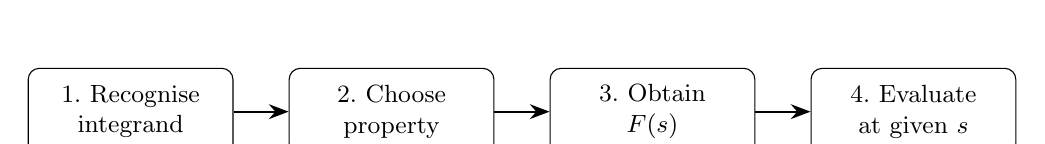
\begin{tikzpicture}[
			node distance=7mm,
			box/.style={rectangle, draw, rounded corners, align=center, minimum width=2.6cm, minimum height=1.1cm, font=\small},
			arr/.style={-{Stealth[length=2.5mm]}, thick}]
			\node[box] (a) {1.\ Recognise\\ integrand};
			\node[box, right=of a] (b) {2.\ Choose\\ property};
			\node[box, right=of b] (c) {3.\ Obtain\\ $F(s)$};
			\node[box, right=of c] (d) {4.\ Evaluate\\ at given $s$};
			\draw[arr] (a)--(b);
			\draw[arr] (b)--(c);
			\draw[arr] (c)--(d);
		\end{tikzpicture}
		\caption{Solution procedure used for all six integrals}
		\label{fig:flow}
	\end{figure}
	
	\subsection{Implementation and Code}
	
	\subsubsection{Mathematical model}
	
	The model is the closed-form transform~\eqref{eq:key}. No iteration is needed to evaluate it. Numerical work enters in only two places: (i) verification of each exact value by adaptive numerical quadrature of the original improper integral, and (ii) analysis of the truncation error of the series used in Proof~2.
	
	\subsubsection{Step size, iteration count, and error estimation}
	
	Truncating the series for $\erf(\sqrt{t})$ after the term $k=N$ gives the partial sum
	\[
	S_N(t)=\frac{2}{\sqrt{\pi}}\sum_{k=0}^{N}\frac{(-1)^k\,t^{\,k+1/2}}{k!\,(2k+1)} .
	\]
	For fixed $t$, the terms $a_k(t)=\tfrac{2}{\sqrt{\pi}}\,t^{k+1/2}/\bigl(k!\,(2k+1)\bigr)$ are eventually decreasing in magnitude and alternate in sign. By the alternating-series estimate, the error is then bounded by the first omitted term:
	\begin{equation}\label{eq:bound}
		\bigl|\erf(\sqrt{t})-S_N(t)\bigr|\le a_{N+1}(t),
	\end{equation}
	valid once $a_k(t)$ is decreasing, which holds for all $k\ge 0$ when $t\le 1$. Table~\ref{tab:partial} applies this to $t=1$, where $\erf(1)=0.8427008$. The tolerance chosen for this check is $10^{-6}$, which is reached at $N=8$.
	
	\begin{table}[htbp]
		\centering
		\caption{Partial sums $S_N(1)$ of the Maclaurin series and the error bound~\eqref{eq:bound}}
		\label{tab:partial}
		\renewcommand{\arraystretch}{1.15}
		\begin{tabular}{rccc}
			\toprule
			$N$ & $S_N(1)$ & Actual error $|\erf(1)-S_N(1)|$ & Bound $a_{N+1}(1)$ \\
			\midrule
			0 & 1.128379 & $2.86\times10^{-1}$ & $3.76\times10^{-1}$ \\
			1 & 0.752253 & $9.04\times10^{-2}$ & $1.13\times10^{-1}$ \\
			2 & 0.865091 & $2.24\times10^{-2}$ & $2.69\times10^{-2}$ \\
			3 & 0.838225 & $4.48\times10^{-3}$ & $5.22\times10^{-3}$ \\
			4 & 0.843449 & $7.48\times10^{-4}$ & $8.55\times10^{-4}$ \\
			5 & 0.842594 & $1.07\times10^{-4}$ & $1.21\times10^{-4}$ \\
			6 & 0.842714 & $1.34\times10^{-5}$ & $1.49\times10^{-5}$ \\
			7 & 0.842699 & $1.50\times10^{-6}$ & $1.65\times10^{-6}$ \\
			8 & 0.842701 & $1.50\times10^{-7}$ & $1.64\times10^{-7}$ \\
			\bottomrule
		\end{tabular}
	\end{table}
	
	For the numerical check of the six integrals, each integrand was evaluated with an adaptive quadrature routine at 20-digit working precision over a subdivided interval $[0,\infty)$. Nested integrals (Examples~\ref{ex:4} and~\ref{ex:6}) were evaluated by inner quadrature at each outer node.
	
	\subsubsection{Code excerpts}
	
	The paper is typeset in \LaTeX\ (Gratzer, 2016). Figures are produced by PGFPlots and TikZ, so they are generated at compile time with no external plotting software. The excerpt below produces the transform plot of Figure~\ref{fig:F}.
	
	\begin{lstlisting}
		\begin{axis}[domain=0.5:6, samples=100,
			xlabel={$s$}, ylabel={$F(s)$}]
			\addplot[thick] {1/(x*sqrt(1+x))};
			\addplot[only marks, mark=*] coordinates
			{(1,0.7071) (3,0.1667) (5,0.0816)};
		\end{axis}
	\end{lstlisting}
	
	The complete source is in the accompanying Git repository. Compiling \texttt{main.tex} reproduces every figure and table in this paper.
	
	\subsection{Results and Visualization}
	
	\subsubsection{Graphical results}
	
	Figure~\ref{fig:erf} shows $\erf(\sqrt{t})$ and $\erfc(\sqrt{t})$. The function rises from $0$ with infinite slope at $t=0$ and approaches $1$, in line with Lemma~\ref{lem:erfprops}(c).
	
	\pgfplotstableread[row sep=\\]{
		t erf \\
		0.00 0.00000 \\ 0.25 0.52050 \\ 0.50 0.68269 \\ 0.75 0.77933 \\ 1.00 0.84270 \\
		1.25 0.88615 \\ 1.50 0.91674 \\ 1.75 0.93863 \\ 2.00 0.95450 \\ 2.25 0.96611 \\
		2.50 0.97465 \\ 2.75 0.98098 \\ 3.00 0.98569 \\ 3.25 0.98921 \\ 3.50 0.99185 \\
		3.75 0.99383 \\ 4.00 0.99532 \\ 4.25 0.99645 \\ 4.50 0.99730 \\ 4.75 0.99795 \\
		5.00 0.99843 \\ 5.25 0.99881 \\ 5.50 0.99909 \\ 5.75 0.99930 \\ 6.00 0.99947 \\
		6.25 0.99959 \\ 6.50 0.99969 \\ 6.75 0.99976 \\ 7.00 0.99982 \\ 7.25 0.99986 \\
		7.50 0.99989 \\ 7.75 0.99992 \\ 8.00 0.99994 \\ 8.25 0.99995 \\ 8.50 0.99996 \\
		8.75 0.99997 \\ 9.00 0.99998 \\
	}\erfdata
	
	\begin{figure}[htbp]
		\centering
		\begin{tikzpicture}
			\begin{axis}[width=0.85\linewidth, height=6cm, xlabel={$t$}, ylabel={value},
				xmin=0, xmax=9, ymin=0, ymax=1.05, grid=major,
				legend style={at={(0.97,0.5)}, anchor=east}, legend cell align=left]
				\addplot[thick, blue] table[x=t, y=erf] {\erfdata};
				\addlegendentry{$\erf(\sqrt{t})$}
				\addplot[thick, red, dashed] table[x=t, y expr=1-\thisrow{erf}] {\erfdata};
				\addlegendentry{$\erfc(\sqrt{t})$}
			\end{axis}
		\end{tikzpicture}
		\caption{The functions $\erf(\sqrt{t})$ and $\erfc(\sqrt{t})$ on $0\le t\le 9$}
		\label{fig:erf}
	\end{figure}
	
	Figure~\ref{fig:F} plots the transform $F(s)=1/(s\sqrt{s+1})$ and marks the values $s=1,3,5$ used in Examples~\ref{ex:1}, \ref{ex:2}, and~\ref{ex:6}.
	
	\begin{figure}[htbp]
		\centering
		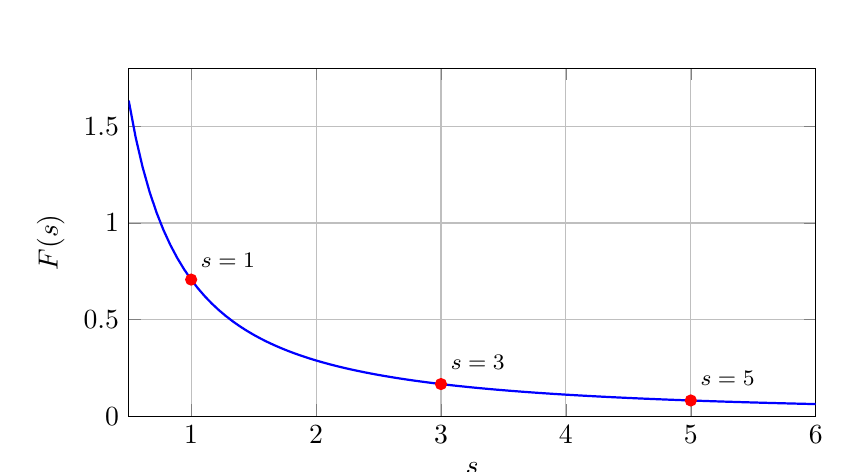
\begin{tikzpicture}
			\begin{axis}[width=0.85\linewidth, height=6cm, xlabel={$s$}, ylabel={$F(s)$},
				xmin=0.5, xmax=6, ymin=0, ymax=1.8, grid=major]
				\addplot[thick, blue, domain=0.5:6, samples=100] {1/(x*sqrt(1+x))};
				\addplot[only marks, mark=*, red] coordinates {(1,0.70711) (3,0.16667) (5,0.08165)};
				\node[anchor=south west, font=\footnotesize] at (axis cs:1,0.72) {$s=1$};
				\node[anchor=south west, font=\footnotesize] at (axis cs:3,0.19) {$s=3$};
				\node[anchor=south west, font=\footnotesize] at (axis cs:5,0.11) {$s=5$};
			\end{axis}
		\end{tikzpicture}
		\caption{The transform $F(s)=\Lap{\erf(\sqrt{t})}$ with the evaluation points $s=1,3,5$}
		\label{fig:F}
	\end{figure}
	
	Figure~\ref{fig:conv} shows the convergence behaviour of the series. The error falls by roughly an order of magnitude per added term and stays below the bound~\eqref{eq:bound}.
	
	\begin{figure}[htbp]
		\centering
		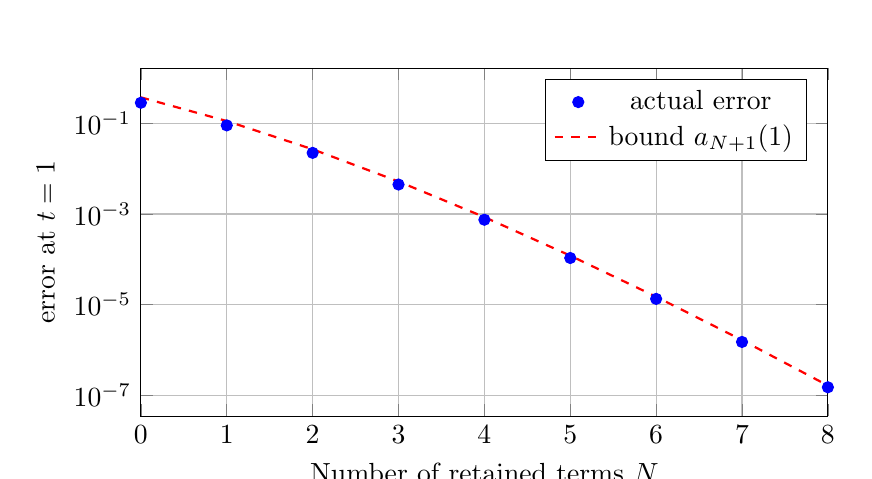
\begin{tikzpicture}
			\begin{semilogyaxis}[width=0.85\linewidth, height=6cm, xlabel={Number of retained terms $N$},
				ylabel={error at $t=1$}, xmin=0, xmax=8, grid=major,
				legend pos=north east]
				\addplot[only marks, mark=*, blue] coordinates
				{(0,0.285678) (1,0.090448) (2,0.022390) (3,0.004476) (4,0.000748)
					(5,0.000107) (6,0.0000134) (7,0.0000015) (8,0.00000015)};
				\addlegendentry{actual error}
				\addplot[thick, red, dashed, domain=0:8, samples=9] {1.128379/(factorial(x+1)*(2*x+3))};
				\addlegendentry{bound $a_{N+1}(1)$}
			\end{semilogyaxis}
		\end{tikzpicture}
		\caption{Truncation error of the Maclaurin series of $\erf(\sqrt{t})$ at $t=1$}
		\label{fig:conv}
	\end{figure}
	
	\subsubsection{Evaluation of the six integrals}
	
	\begin{example}\label{ex:1}
		Evaluate $I_1=\displaystyle\int_0^\infty e^{-t}\erf(\sqrt{t})\dd t$.
		
		By Definition~\ref{def:laplace} with $f(t)=\erf(\sqrt{t})$ and $s=1$, $I_1=F(1)=\dfrac{1}{1\cdot\sqrt{2}}=\dfrac{1}{\sqrt{2}}$.
	\end{example}
	
	\begin{example}\label{ex:2}
		Evaluate $I_2=\displaystyle\int_0^\infty t\,e^{-3t}\erf(\sqrt{t})\dd t$.
		
		Multiplication by $t$ gives $\Lap{t\,\erf(\sqrt{t})}=-F'(s)$. Differentiating $F(s)=s^{-1}(1+s)^{-1/2}$,
		\[
		F'(s)=-\frac{1}{s^2\sqrt{1+s}}-\frac{1}{2s(1+s)^{3/2}}=-\frac{2(1+s)+s}{2s^2(1+s)^{3/2}}=-\frac{2+3s}{2s^2(1+s)^{3/2}} .
		\]
		Hence
		\begin{equation}\label{eq:tF}
			\Lap{t\,\erf(\sqrt{t})}=\frac{2+3s}{2s^2(1+s)^{3/2}} .
		\end{equation}
		At $s=3$: $I_2=\dfrac{11}{2\cdot 9\cdot 8}=\dfrac{11}{144}$.
	\end{example}
	
	\begin{example}\label{ex:3}
		Evaluate $I_3(s)=\displaystyle\int_0^\infty e^{-(s-2)t}\erf(\sqrt{t})\dd t$.
		
		The integrand is $e^{-(s-2)t}f(t)$, which is the transform $F$ at $s-2$. Equivalently, the first shifting property with $a=2$ gives $\Lap{e^{2t}\erf(\sqrt{t})}=F(s-2)$. Therefore
		\[
		I_3(s)=\frac{1}{(s-2)\sqrt{s-1}},\qquad s>2 .
		\]
		The condition $s>2$ is required for convergence because $s-2$ must be positive. As an illustration, $s=4$ gives $I_3(4)=\dfrac{1}{2\sqrt{3}}\approx 0.288675$.
	\end{example}
	
	\begin{example}\label{ex:4}
		Evaluate $I_4=\displaystyle\int_0^\infty e^{-t}\left\{\int_0^t \erf(\sqrt{u})\dd u\right\}\dd t$.
		
		By the integral property, $\Lap{\int_0^t\erf(\sqrt{u})\dd u}=\dfrac{F(s)}{s}=\dfrac{1}{s^2\sqrt{1+s}}$. At $s=1$, $I_4=\dfrac{1}{\sqrt{2}}$.
	\end{example}
	
	\begin{example}\label{ex:5}
		Evaluate $I_5=\displaystyle\int_0^\infty e^{-2t}\,\frac{\dd}{\dd t}\erf(2\sqrt{t})\dd t$.
		
		Since $\erf(2\sqrt{t})=f(4t)$, the change-of-scale property with $a=4$ gives
		\[
		\Lap{\erf(2\sqrt{t})}=\frac{1}{4}F\!\left(\frac{s}{4}\right)=\frac{1}{4}\cdot\frac{1}{\tfrac{s}{4}\sqrt{1+\tfrac{s}{4}}}=\frac{2}{s\sqrt{s+4}} .
		\]
		The derivative property, with $\erf(0)=0$, gives $\Lap{\tfrac{\dd}{\dd t}\erf(2\sqrt{t})}=\dfrac{2}{\sqrt{s+4}}$. At $s=2$, $I_5=\dfrac{2}{\sqrt{6}}=\sqrt{\dfrac{2}{3}}$.
	\end{example}
	
	\begin{example}\label{ex:6}
		Evaluate $I_6=\displaystyle\int_0^\infty e^{-5t}\bigl[\erf\sqrt{t}*\erf\sqrt{t}\bigr]\dd t$.
		
		By the convolution theorem, $\Lap{\erf\sqrt{t}*\erf\sqrt{t}}=F(s)^2=\dfrac{1}{s^2(1+s)}$. At $s=5$, $I_6=\dfrac{1}{25\cdot 6}=\dfrac{1}{150}$.
	\end{example}
	
	Table~\ref{tab:results} compares each exact value with the independent numerical computation.
	
	\begin{table}[htbp]
		\centering
		\caption{Exact values from the Laplace transform method versus numerical quadrature}
		\label{tab:results}
		\small
		\renewcommand{\arraystretch}{1.5}
		\resizebox{\linewidth}{!}{%
			\begin{tabular}{@{}c l l c c c@{}}
				\toprule
				No. & Improper integral & Property used & $s$ & Exact value & Numerical \\
				\midrule
				1 & $\displaystyle\int_0^\infty e^{-t}\erf(\sqrt{t})\dd t$ & Definition & 1 & $1/\sqrt{2}\approx 0.707107$ & 0.707107 \\
				2 & $\displaystyle\int_0^\infty t\,e^{-3t}\erf(\sqrt{t})\dd t$ & Multiplication by $t$ & 3 & $11/144\approx 0.076389$ & 0.076389 \\
				3 & $\displaystyle\int_0^\infty e^{-(s-2)t}\erf(\sqrt{t})\dd t$ & First shifting & 4 & $1/(2\sqrt{3})\approx 0.288675$ & 0.288675 \\
				4 & $\displaystyle\int_0^\infty e^{-t}\!\left\{\int_0^t\erf(\sqrt{u})\dd u\right\}\dd t$ & Integral & 1 & $1/\sqrt{2}\approx 0.707107$ & 0.707107 \\
				5 & $\displaystyle\int_0^\infty e^{-2t}\tfrac{\dd}{\dd t}\erf(2\sqrt{t})\dd t$ & Scale and derivative & 2 & $\sqrt{2/3}\approx 0.816497$ & 0.816497 \\
				6 & $\displaystyle\int_0^\infty e^{-5t}\bigl[\erf\sqrt{t}*\erf\sqrt{t}\bigr]\dd t$ & Convolution & 5 & $1/150\approx 0.006667$ & 0.006667 \\
				\bottomrule
		\end{tabular}}
	\end{table}
	
	All six values reported by Aggarwal et al.\ (2019) are confirmed. The value of $I_3$ in the article is left as a function of $s$ and is checked here at $s=4$. Examples~\ref{ex:1} and~\ref{ex:4} share the value $1/\sqrt{2}$ only because they are both evaluated at $s=1$, where division by $s$ in the integral property changes nothing.
	
	\subsection{Analysis and Discussion}
	
	\subsubsection{Accuracy, convergence, and stability}
	
	The Laplace transform method is exact: once Equation~\eqref{eq:key} is established, each integral reduces to evaluating an algebraic expression, so no truncation or quadrature error enters the result. The numerical agreement in Table~\ref{tab:results} supports the algebra rather than measuring the method's accuracy.
	
	Convergence is the delicate point. The transform integral~\eqref{eq:laplace} converges only for $s$ above a threshold, and every property of Table~\ref{tab:properties} shifts or rescales that threshold. For $F(s)=1/(s\sqrt{s+1})$ the threshold is $s>0$. In Example~\ref{ex:3} the shift moves it to $s>2$. The series derivation is also sensitive to $s$: the binomial series converges only for $s>1$, yet Examples~\ref{ex:1} and~\ref{ex:4} use $s=1$, on the boundary. The final values remain valid because Proof~1 establishes the formula for all $s>0$, but the series argument alone does not justify them.
	
	\subsubsection{Computational cost and practical significance}
	
	The method requires one derivation of the base transform, after which each integral costs a few algebraic steps. Direct numerical quadrature of an integral over $[0,\infty)$ needs interval subdivision or a variable transformation and, for nested integrals, repeated inner integration. The practical value of the method is that a single formula serves a whole family of integrals, and the parameter $s$ remains symbolic until the last step.
	
	\subsubsection{Peer review of Aggarwal et al.\ (2019)}
	
	\textit{Strengths.} The article states its goal clearly, lists the properties it needs before applying them, and chooses examples that exercise a different property each time. All six numerical results are correct. The core transform~\eqref{eq:key} is also correct.
	
	\textit{Weaknesses.} The review found the following errors and omissions, listed in Table~\ref{tab:errors}.
	
	\begin{table}[htbp]
		\centering
		\caption{Errors and omissions found in Aggarwal et al.\ (2019)}
		\label{tab:errors}
		\small
		\renewcommand{\arraystretch}{1.3}
		\begin{tabular}{@{}c p{4.2cm} p{4.5cm} p{4.2cm}@{}}
			\toprule
			No. & Location and statement in the article & Problem & Correction \\
			\midrule
			1 & Page 3, properties list: $\erfc(x)\to 1$ as $x\to\infty$ & Contradicts $\erfc=1-\erf$ and $\erf\to 1$ & $\erfc(x)\to 0$ as $x\to\infty$ \\
			2 & Equation (11): $\Lap{t\,\erf(\sqrt{t})}=-\dfrac{2+s}{2s^2(1+s)^{3/2}}$ & Wrong sign and wrong numerator; the next lines use $2+3s$ with a positive sign & $\dfrac{2+3s}{2s^2(1+s)^{3/2}}$, as in Equation~\eqref{eq:tF} \\
			3 & Page 2, change of scale: $\Lap{e^{at}F(at)}=\tfrac{1}{a}f\!\left(\tfrac{s}{a}\right)$ & Mixes the shifting and scaling properties; the example actually uses the scaling rule alone & $\Lap{F(at)}=\tfrac{1}{a}f\!\left(\tfrac{s}{a}\right)$ \\
			4 & Examples 1, 4: $s=1$; Example 3: $s$ unrestricted & No convergence conditions are stated; the series derivation holds only for $s>1$; Example 3 needs $s>2$ & State the region of convergence for each example \\
			5 & First page: ``Issue 2''; running headers: ``Issue 1'' & Inconsistent publication details & Use Volume 4, Issue 2 consistently \\
			6 & Text of the introduction: ``complimentary'' error function & Wrong word & ``complementary'' \\
			\bottomrule
		\end{tabular}
	\end{table}
	
	None of these errors affects the six final values. Items 1 and 2 are the most consequential for a reader, because a student who copies Equation~(11) will obtain a negative value for a positive integral. Item 4 is the main mathematical gap: the article offers no justification for interchanging summation and integration and no reason for the chosen values of $s$.
	
	\subsubsection{Limitations and assumptions}
	
	The method works only when the integrand can be matched to a known transform through one of the listed properties. It is also confined to arguments of the form $\erf(a\sqrt{t})$. Integrals such as $\int_0^\infty e^{-st}\erf(t)\dd t$ require a different base transform. The numerical verification in this paper covers only the parameter values shown, not the full range of $s$.
	
	\section{Conclusion}
	
	This paper re-derived the Laplace transform of $\erf(\sqrt{t})$, obtaining $1/(s\sqrt{s+1})$ for all $s>0$, and used it with six standard properties to evaluate the six improper integrals of Aggarwal et al.\ (2019). Every value was confirmed by independent numerical quadrature, and the truncation error of the underlying series was shown to follow the alternating-series bound. The method is exact, short, and reusable across a family of integrals.
	
	The review also found that the article contains notational and logical lapses: a wrong limit for $\erfc$, an incorrect transform of $t\,\erf(\sqrt{t})$, a misstated change-of-scale property, missing convergence conditions, and inconsistent publication details. These do not change the final answers, but they reduce the article's reliability as a teaching source. The main lesson for Advanced Calculus is that a transform method is only as sound as the stated region of convergence on which it is applied.
	
	\subsection{Possible Extensions}
	
	Several directions follow naturally from this work:
	\begin{enumerate}[label=\arabic*.]
		\item deriving the transform of $\erf(a\sqrt{t})$ and of $\erfc(a/\sqrt{t})$, which occur in heat-conduction solutions;
		\item applying the same procedure to related special functions, such as Bessel functions;
		\item comparing the Laplace method with other integral transforms, such as the Mahgoub or Sumudu transforms discussed by Aggarwal et al.\ (2019); and
		\item publishing a reproducible numerical-verification script alongside the \LaTeX\ source so that every table of values can be regenerated by readers.
	\end{enumerate}
	
	\newpage
	\begin{thebibliography}{99}
		
		\bibitem{aggarwal2019}
		Aggarwal, S., Singh, A., Kumar, A., \& Kumar, N. (2019). Application of Laplace transform for solving improper integrals whose integrand consisting error function. \textit{Journal of Advanced Research in Applied Mathematics and Statistics}, \textit{4}(2), 1--7.
		
		\bibitem{debnath2006}
		Debnath, L., \& Bhatta, D. (2006). \textit{Integral transforms and their applications} (2nd ed.). Chapman \& Hall/CRC.
		
		\bibitem{gratzer2016}
		Gr\"atzer, G. (2016). \textit{More math into \LaTeX}. Springer. \url{https://doi.org/10.1007/978-3-319-23796-1}
		
		\bibitem{korn2000}
		Korn, G. A., \& Korn, T. M. (2000). \textit{Mathematical handbook for scientists and engineers: Definitions, theorems, and formulas for reference and review}. Dover Publications.
		
		\bibitem{zill2016}
		Zill, D. G. (2016). \textit{Advanced engineering mathematics}. Jones \& Bartlett Learning.
		
	\end{thebibliography}
	
	\newpage
	\appendix
	\section{Verification of Equation~\eqref{eq:tF} at $s=3$}
	
	For completeness, the arithmetic of Example~\ref{ex:2} is shown in full. With $s=3$,
	\[
	\frac{2+3s}{2s^2(1+s)^{3/2}}=\frac{2+9}{2\cdot 9\cdot 4^{3/2}}=\frac{11}{18\cdot 8}=\frac{11}{144}\approx 0.076389 .
	\]
	The same value was obtained by numerical quadrature of $\int_0^\infty t\,e^{-3t}\erf(\sqrt{t})\dd t$ (Table~\ref{tab:results}), which confirms the corrected form of Equation~(11) of Aggarwal et al.\ (2019). The value obtained from their printed Equation~(11), $-\tfrac{2+3}{2\cdot 9\cdot 8}=-\tfrac{5}{144}$, is negative and cannot equal the integral of a positive integrand.
	
\end{document}